\subchapter{Advanced Yocto configuration}{Configure the build, customize the
	output images and use NFS}

During this lab, you will:
\begin{itemize}
  \item Customize the package selection
  \item Configure the build system
  \item Use the rootfs over NFS
\end{itemize}

\section{Set up the Ethernet communication}

Later on, we will mount our root filesystem through the network using
NFS. This works on top of an Ethernet connection.

With a network cable, connect the Ethernet port of your board to the
one of your computer. If your computer already has a wired connection
to the network, your instructor will provide you with a USB Ethernet
adapter. A new network interface, probably \code{eth1} or \code{eth2},
should appear on your Linux system.

To configure this network interface on the workstation side, click on
the {\em Network Manager} tasklet on your desktop, and select {\em
Edit Connections}.

\begin{center}
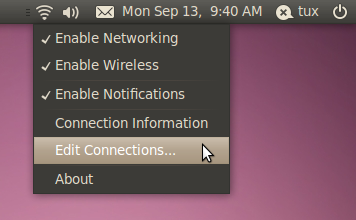
\includegraphics[width=8cm]{../labs/yocto-advanced-configuration/network-config-1.png}
\end{center}

Select the new {\em wired network connection}:

\begin{center}
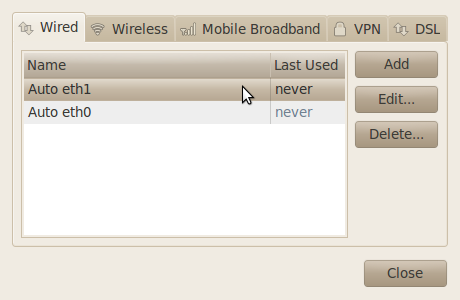
\includegraphics[width=8cm]{../labs/yocto-advanced-configuration/network-config-2.png}
\end{center}

In the \code{IPv4 Settings} tab, press the \code{Add} button
and make the interface use a static IP
address, like \code{192.168.0.1} (of course, make sure that this
address belongs to a separate network segment from the one of the main
company network).

\begin{center}
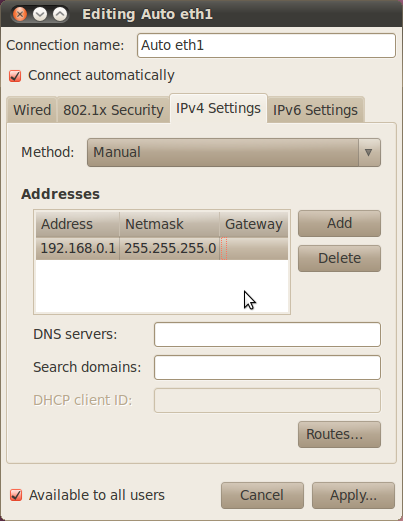
\includegraphics[width=8cm]{../labs/yocto-advanced-configuration/network-config-3.png}
\end{center}

You can use \code{255.255.255.0} as \code{Netmask}, and leave the
\code{Gateway} field untouched (if you click on the \code{Gateway} box, you
will have to type a valid IP address, otherwise you won't be apply to
click on the \code{Apply} button).

Now, configure the network on the board in U-Boot by setting the \code{ipaddr}
and \code{serverip} environment variables:

\begin{verbatim}
setenv ipaddr 192.168.0.100
setenv serverip 192.168.0.1
\end{verbatim}

The first time you use your board, you also need to send the MAC address
in U-boot:

\begin{verbatim}
setenv ethaddr 12:34:56:ab:cd:ef
\end{verbatim}

In case the board was previously configured in a different way, we
also turn off automatic booting after commands that can be used to
copy a kernel to RAM:

\begin{verbatim}
setenv autostart no
\end{verbatim}

To make these settings permanent, save the environment:

\begin{verbatim}
saveenv
\end{verbatim}

Now switch your board off and on again\footnote{Power cycling your
board is needed to make your \code{ethaddr} permanent, for obscure
reasons. If you don't, U-boot will complain that \code{ethaddr} is not
set.}.

\section{Set up the NFS server}

First install the NFS server on the training computer and create the root NFS
directory:
\begin{verbatim}
sudo apt-get install nfs-kernel-server
sudo mkdir -m 777 /nfs
\end{verbatim}

Then make sure this directory is used and exported by the NFS server by adding
\code{/nfs *(rw,sync,no_root_squash,subtree_check)} to the
\code{/etc/exports} file.

Finally restart the service:
\begin{verbatim}
sudo service nfs-kernel-server restart
\end{verbatim}

\section{Tell the kernel to use the rootfs over NFS}

Then set the kernel boot arguments U-Boot will pass to the Linux kernel at boot
time:
\begin{verbatim}
setenv bootargs 'console=ttyO0 root=/dev/nfs rw nfsroot=192.168.0.1:/nfs
  ip=192.168.0.100'
saveenv
\end{verbatim}

If you later want to make changes to this setting, you can use:
\begin{verbatim}
editenv bootargs
\end{verbatim}

\section{Add a package to the rootfs image}

You can add packages to be built by editing the local configuration file
\code{$BUILDDIR/conf/local.conf}. The \code{IMAGE_INSTALL} variable controls the
packages included into the output image.

To illustrate this, add the Dropbear SSH server to the list of enabled
packages.

Tip: do not override the default enabled package list, but append the Dropbear
package instead.

\section{Choose a package variant}

Dependencies of a given package are explicitly defined in its recipe.
Some packages may need a specific library or piece of software but
others only depend on a functionality. As an example, the kernel
dependency is described by \code{virtual/kernel}.

To see which kernel is used, dry-run BitBake:
\begin{verbatim}
bitbake -vn virtual/kernel
\end{verbatim}

In our case, we can see the \code{linux-ti-staging} provides the
\code{virtual/kernel} functionality:
\small
\begin{verbatim}
NOTE: selecting linux-ti-staging to satisfy virtual/kernel due to PREFERRED_PROVIDER
\end{verbatim}
\normalsize

We can force Yocto to select another \code{kernel} by explicitly
defining which one to use in our local configuration. Try switching
from \code{linux-ti-staging} to \code{linux-dummy} only using the
local configuration.

Then check the previous step worked by dry-running again BitBake.
\begin{verbatim}
bitbake -vn virtual/kernel
\end{verbatim}

You can now rebuild the whole Yocto project, with \code{bitbake
core-image-minimal}

Tip: you need to define the more specific information here to be sure it is the
one used. The \code{MACHINE} variable can help here.

As this was only to show how to select a preferred provider for a
given package, you can now use \code{linux-ti-staging} again.

\section{Boot with the updated rootfs}

First we need to put the rootfs under the NFS root directory so that it is
accessible by NFS clients. Simply uncompress the archived output image in the
previously created \code{/nfs} directory:
\begin{verbatim}
tar xpf $BUILDDIR/tmp/deploy/images/beaglebone/\
  core-image-minimal-beaglebone.tar.gz -C /nfs
\end{verbatim}

Then boot the board.

The Dropbear SSH server was enabled a few steps before, and should now be
running as a service on the BeagleBone Black. You can test it by accessing the
board through SSH:
\begin{verbatim}
ssh root@192.168.0.100
\end{verbatim}

You should see the BeagleBone Black command line!

\section{Going further: BitBake tips}

BitBake is a powerful tool which can be used to execute specific commands. Here
is a list of some useful ones, used with the \code{virtual/kernel} package.

\begin{itemize}
  \item The Yocto recipes are divided into numerous tasks, you can print them
        by using: \code{bitbake -c listtasks virtual/kernel}.
  \item BitBake allows to call a specific task only (and its dependencies)
        with: \code{bitbake -c <task> virtual/kernel}. (\code{<task>} can be
        \code{menuconfig} here).
  \item You can force to rebuild a package by calling: \code{bitbake -f
        virtual/kernel}
  \item \code{world} is a special keyword for all packages. \code{bitbake -c
        fetchall world} will download all packages sources (and their
        dependencies).
  \item You can get a list of locally available packages and their current
        version with: \\
        \code{bitbake -s}
  \item You can also find detailed information on available packages, their
        current version, dependencies or the contact information of the
        maintainer by visiting: \\
        \url{http://packages.yoctoproject.org/}
\end{itemize}

For detailed information, please run \code{bitbake -h}
